\section{Disambiguation}

\begin{frame}[fragile]
	\frametitle{Field Symmetry Disambiguation Idea}
	
	\Large
	
	\vspace{0.3cm}
	
	\begin{itemize}
		\item Each player \textbf{is able} to give an estimation of different global target
			  positions on the field (i.e., localization)
		\vspace{0.2cm}
		\item Exploiting the \emph{PTracking} method, it is \textbf{possible to compare} the
			  target positions perceived by a single robot with the ones given by the data
			  fusion algorithm
	\end{itemize}
	
	\vspace{-0.4cm}
	
	\begin{center}
		\Huge
		
		\textcolor{red}{\textbf{$ \Downarrow $}}
	\end{center}
	
	\vspace{-0.2cm}
	
	\begin{verbbox}
		if (signsDiff(ownBallPos,fusedBallPos) &&
		   (modulesSim(ownBallPos,fusedBallPos)) {
   ... \* Invert Signs *\
		}
	\end{verbbox}
	
	\begin{figure}[!H]
		\centering
		\theverbbox
	\end{figure}
\end{frame}

\begin{frame}
	\frametitle{Field Symmetry Disambiguation}
	
	\Large
	
	Analyzing this idea two main problems can be identified:
	
	\begin{enumerate}
		\item The algorithm could not work if the majority of the teammates are not correctly
			  localized (depending on the localization covariance matrices)
		\vspace{0.2cm}
		\item The error given by the image processor could cause fluctuations of the estimation
			  signs near the field lines of symmetry
	\end{enumerate}
\end{frame}

\begin{frame}
	\frametitle{Field Symmetry Disambiguation}
	
	\Large
	
	\vspace{0.08cm}
	
	\begin{enumerate}
		\item The first problem can be partially addressed by using different weights on the
			  players (e.g., goalie)
		
		\seti
	\end{enumerate}
	
	\begin{columns}[T]
		\column{.468\textwidth}
		
		\begin{enumerate}
			\vspace{-0.4cm}
			\conti
			\item The second one can be overcome by dividing the field in four zones:
				  
				  \begin{itemize}
				  	  \item \textbf{Zone 1:} no instability problems
				  	  \vspace{0.15cm}
				  	  \item \textbf{Zone 2:} considering only the X coord
				  	  \vspace{0.15cm}
				  	  \item \textbf{Zone 3:} considering only the Y coord
				  	  \vspace{0.15cm}
				  	  \item \textbf{Zone 4:} still instability
				  \end{itemize}
		\end{enumerate}
		
		\column{.5\textwidth}
		\centering
		
		\vspace{0.25cm}
		
		\begin{tikzpicture}
			\node at (0,0) [draw=white,ultra thick,inner sep=0pt]
			{
				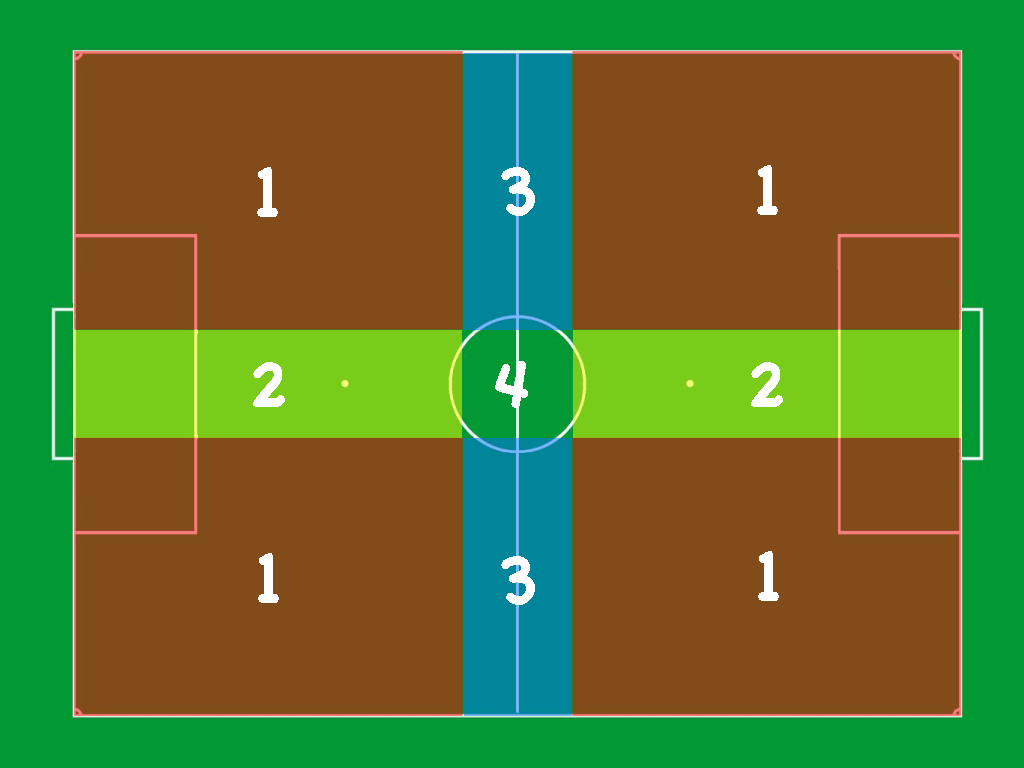
\includegraphics[width=6cm]{Figures/SoccerField}
			};
		\end{tikzpicture}
	\end{columns}
\end{frame}
